\chapter{L'atome d'hydrogène}\label{ch:b3:hydrogen-atom}

Neuf atomes sur dix dans l'univers sont de l'hydrogène~: un proton qui
retient un électron, le seul atome que la physique sache résoudre
exactement --- et la clé qui a ouvert tous les autres. L'ancienne
théorie des quanta du \cref{ch:b3:hamiltonian-mechanics} devinait ses
énergies~; la machinerie est désormais en place pour les
\emph{obtenir}~: le potentiel coulombien entre dans l'\omterm{prop:b3:schrodinger-three-dimensions:swave}{équation radiale}
du chapitre précédent, et il en sort les niveaux $-E_{\text{I}}/n^2$,
le \omterm{thm:b3:hydrogen-atom:levels}{rayon de Bohr}, les couches et sous-couches du tableau périodique de
la chimie, et les séries spectrales que les astronomes lisent dans
chaque nébuleuse. La même solution, réétalonnée, décrit l'hélium
ionisé, les atomes muoniques, le positronium et les «~atomes~»
électron--trou des semi-conducteurs~; étirée jusqu'à $n
\approx 100$ elle décrit les atomes de Rydberg d'un demi-micromètre,
dont les chuchotements radio cartographient les nuages ionisés de la
Galaxie et dont les interactions font aujourd'hui tourner des
ordinateurs quantiques.
% NOTE: full radial solutions (Laguerre) admitted; ground state solved
% exactly; emphasis on scaling laws and applications.

\section{Le problème de Coulomb résolu}

\begin{theorem}[Niveaux de l'hydrogène]\label{thm:b3:hydrogen-atom:levels}
\index{atome d'hydrogène}\index{nombre quantique principal}\index{rayon de Bohr}
Pour $V(r) = -e^2/4\pi\varepsilon_0 r$ (on pose $k = e^2/4\pi
\varepsilon_0$), les états liés sont étiquetés $(n, l, m)$ avec
\[
E_n = -\frac{E_{\text{I}}}{n^2} , \qquad
E_{\text{I}} = \frac{m_{\text{e}}k^2}{2\hbar^2} = \qty{13.6}{eV} ,
\qquad n = 1, 2, 3, \dots
\]
et, pour chaque $n$, les nombres orbitaux $l = 0, 1, \dots, n-1$ et
$m = -l, \dots, l$. La longueur naturelle est le \omterm{thm:b3:hydrogen-atom:levels}{rayon de Bohr} $a_0 =
\hbar^2/m_{\text{e}}k = \qty{52.9}{pm}$~; l'état fondamental s'écrit
\[
\psi_{100} = \frac{1}{\sqrt{\pi a_0^3}}\;\eu^{-r/a_0} .
\]
L'énergie dépend de $n$ \emph{seul}~: en comptant les $m$ et les $l$,
le niveau $n$ est $n^2$ fois dégénéré (le double avec le spin,
\cref{ch:b3:spin-two-level}) --- bien au-delà de la dégénérescence
$(2l+1)$ que l'isotropie explique.
\end{theorem}

\begin{proof}[Démonstration partielle]
Pour l'état fondamental, essayons $u = Cr\,\eu^{-r/a}$ dans l'\omterm{prop:b3:schrodinger-three-dimensions:swave}{équation
radiale} avec $l = 0$~: $u'' = (1/a^2 - 2/ar)u$, si bien que
$-\tfrac{\hbar^2}{2m_{\text{e}}}u'' - \tfrac kr u = Eu$ exige
$\hbar^2/m_{\text{e}}a = k$ (en identifiant les termes en $1/r$) ---
c'est-à-dire $a = a_0$ --- et $E = -\hbar^2/2m_{\text{e}}a_0^2 = -E_{\text{I}}$.
La solution générale (polynômes de Laguerre, $n - l - 1$ nœuds
radiaux) est admise~; chaque étape de la construction est élémentaire
mais longue. La dégénérescence «~accidentelle~» en $l$ reflète un
secret classique de la force en $1/r$ pure --- les ellipses de Kepler
ne précessent pas, et un vecteur conservé supplémentaire
(Laplace--Runge--Lenz) pointe le long du grand axe fixe~; sa version
quantique est ce qui relie des $l$ différents à une même énergie
(\cref{exo:b3:hydrogen-atom:12}).
\end{proof}

\begin{omfigure}
\begin{tikzpicture}[font=\small, >=Stealth]
  % energy scale: E = -13.6/n^2, map E -> y = 5.6 + E*0.42 (E in eV)
  % n=1: y=-0.11? choose y(E) = 5.9 + 0.42*E: n1: 0.19, n2: 4.47, n3: 5.27, n4: 5.55, inf: 5.9
  \draw[->] (-0.4,-0.4) -- (-0.4,6.6);
  \node[anchor=south] at (-0.4,6.6) {$E$ (eV)};
  % continuum
  \fill[gray!15] (0,5.9) rectangle (8.6,6.45);
  \node[anchor=west, font=\footnotesize] at (8.7,6.15) {continuum~: atome ionisé};
  \draw[thick] (0,5.9) -- (8.6,5.9);
  \node[anchor=east, font=\footnotesize] at (-0.5,5.9) {$0$};
  % levels, split by l columns
  \foreach \n/\y in {1/0.19, 2/4.47, 3/5.27, 4/5.55}
    {\node[anchor=east, font=\footnotesize] at (-0.5,\y) {$-13.6/\n^2$};}
  % l columns: s at x 0-1.4, p at 1.9-3.3, d at 3.8-5.2, f 5.7-7.1
  \node[font=\footnotesize] at (0.7,-0.3) {$l = 0$ ($s$)};
  \node[font=\footnotesize] at (2.6,-0.3) {$l = 1$ ($p$)};
  \node[font=\footnotesize] at (4.5,-0.3) {$l = 2$ ($d$)};
  \node[font=\footnotesize] at (6.4,-0.3) {$l = 3$ ($f$)};
  \draw[very thick, omDef] (0,0.19) -- (1.4,0.19);
  \foreach \x in {0,1.9} \draw[very thick, omDef] (\x,4.47) -- ({\x+1.4},4.47);
  \foreach \x in {0,1.9,3.8} \draw[very thick, omDef] (\x,5.27) -- ({\x+1.4},5.27);
  \foreach \x in {0,1.9,3.8,5.7} \draw[very thick, omDef] (\x,5.55) -- ({\x+1.4},5.55);
  % series arrows
  \draw[->, omExo, thick] (0.5,4.47) -- (0.6,0.24);
  \draw[->, omExo, thick] (1.0,5.27) -- (0.85,0.24);
  \node[omExo, font=\footnotesize, anchor=west] at (0.95,2.3) {Lyman (UV)};
  \draw[->, omThm, thick] (2.6,5.27) -- (2.45,4.52);
  \draw[->, omThm, thick] (3.1,5.55) -- (2.9,4.52);
  \node[omThm, font=\footnotesize, anchor=west] at (3.25,4.95) {Balmer (visible)};
  \node at (1.9,1.55) {};
\end{tikzpicture}

{\small Les niveaux de l'hydrogène $-E_{\text{I}}/n^2$, étalés selon
$l$~: toutes les sous-couches d'un même $n$ coïncident (l'«~accident~»
coulombien). Les sauts descendants qui se terminent sur $n = 1$
forment la \omterm{prop:b3:hydrogen-atom:series}{série de Lyman}, ultraviolette~; ceux qui se terminent sur
$n = 2$, la \omterm{prop:b3:hydrogen-atom:series}{série de Balmer}, visible, qui colore les nébuleuses en
rouge.}
\end{omfigure}

\section{Où se trouve l'électron}

\begin{proposition}[Distributions radiales]\label{prop:b3:hydrogen-atom:radial}
\index{probabilité radiale}
La probabilité de trouver l'électron entre $r$ et $r + \dd r$ vaut
$P(r)\,\dd r$ avec $P(r) = |u(r)|^2$, le carré de la fonction radiale
normée de \cref{thm:b3:quantum-angular-momentum:radial}. Pour les
états les plus bas~: $P_{1s} \propto r^2\eu^{-2r/a_0}$, maximale
exactement en $r = a_0$ avec $\langle r\rangle = \tfrac32 a_0$~;
$P_{2s}$ montre deux bosses séparées par un \emph{nœud} sphérique~; $P_{2p} \propto
r^4\eu^{-r/a_0}$, maximale en $4a_0$. En général $\langle r\rangle
\approx n^2a_0$~: les atomes grandissent \emph{quadratiquement} avec
l'excitation, tandis que leur liaison décroît en $1/n^2$ --- le levier
qui produit les géants de Rydberg de \cref{pb:b3:hydrogen-atom:1}.
\end{proposition}
\admitted

\begin{omfigure}
\begin{tikzpicture}
  \begin{axis}[omaxis, axis x line=bottom, axis y line=left,
    width=11.6cm, height=5.8cm, xmin=0, xmax=14, ymin=0, ymax=0.62,
    xlabel={$r/a_0$}, ylabel={$P(r)$ (par $a_0$)},
    xlabel style={at={(axis description cs:0.5,-0.1)}, anchor=north},
    xtick={1,4,5,10}, ytick=\empty, clip=false,
    legend style={font=\scriptsize, at={(0.95,0.9)}, anchor=north east,
      draw=none, fill=none}]
    \addplot[omDef, very thick, domain=0:8, samples=120] {4*x*x*exp(-2*x)};
    \addlegendentry{$1s$}
    \addplot[omThm, thick, domain=0:14, samples=140] {0.125*x*x*(2-x)^2*exp(-x)};
    \addlegendentry{$2s$}
    \addplot[omExo, thick, domain=0:14, samples=140] {x^4*exp(-x)/24};
    \addlegendentry{$2p$}
    \draw[gray, dashed] (axis cs:1,0) -- (axis cs:1,0.545);
  \end{axis}
\end{tikzpicture}

{\small Densités de \omterm{prop:b3:hydrogen-atom:radial}{probabilité radiale}. Le maximum de $1s$ se situe
exactement en $a_0$~; l'état $2s$ porte un nœud sphérique et un lobe
proche du noyau --- la «~pénétration~» qui ordonnera le tableau
périodique --- tandis que $2p$, muré par la \omterm{thm:b3:quantum-angular-momentum:radial}{barrière centrifuge}, reste
à distance.}
\end{omfigure}

\begin{example}[Lire les tailles]\label{ex:b3:hydrogen-atom:sizes}
État fondamental~: \qty{0.1}{nm} de diamètre, \qty{13.6}{eV} de
profondeur --- les échelles de toute la chimie. À $n = 10$~: rayon
$\sim\qty{5}{nm}$, liaison \qty{0.136}{eV} --- retenu de façon lâche.
À $n = 100$~: un atome de taille \emph{micrométrique} lié par
\qty{1.4}{meV}, détruit par le champ le plus faible --- et pourtant
l'espace interstellaire est assez vide pour que de tels atomes vivent
et émettent (\cref{pb:b3:hydrogen-atom:1}).
\end{example}

\section{Le spectre}

\begin{proposition}[Séries et règles de sélection]\label{prop:b3:hydrogen-atom:series}
\index{série de Balmer}\index{série de Lyman}
Un saut $n' \to n$ émet la longueur d'onde
\[
\frac{1}{\lambda} = R_{\text{H}}\Big(\frac{1}{n^2} -
\frac{1}{n'^2}\Big) , \qquad
R_{\text{H}} = \frac{E_{\text{I}}}{hc} = \qty{1.097e7}{m^{-1}} ,
\]
soumis à la règle de sélection dipolaire $\Delta l = \pm1$ (le photon
emporte $\hbar$). La \omterm{prop:b3:hydrogen-atom:series}{série de Lyman} ($\to n = 1$) se situe dans
l'ultraviolet lointain à partir de \qty{121.6}{nm}~; la \omterm{prop:b3:hydrogen-atom:series}{série de
Balmer} ($\to n = 2$) commence à la raie rouge $H\alpha$,
\qty{656.3}{nm} --- la couleur des nébuleuses en émission et des
protubérances solaires~; les séries de Paschen et suivantes reculent
dans l'infrarouge, et entre $n = 110$ et $109$ la même formule tombe à
\qty{5.0}{GHz}~: l'hydrogène parle de l'ultraviolet au cadran radio.
\end{proposition}

\begin{proof}
Conservation de l'énergie avec \cref{thm:b3:hydrogen-atom:levels}~;
$R_{\text{H}}$ comme dans \cref{pb:b3:hamiltonian-mechanics:1},
désormais obtenu et non plus postulé.
\end{proof}

\begin{example}[Atomes hydrogénoïdes~: une solution, beaucoup d'atomes]\label{ex:b3:hydrogen-atom:scaling}
Remplaçons la charge du proton par $Ze$ et l'électron par une masse en
orbite $\mu$ quelconque~: toute formule se réétalonne selon
\[
a \to a_0\,\frac{m_{\text{e}}}{\mu}\,\frac1Z , \qquad
E_{\text{I}} \to E_{\text{I}}\,\frac{\mu}{m_{\text{e}}}\,Z^2 .
\]
He$^+$ ($Z = 2$)~: \qty{54.4}{eV}. Les électrons internes des atomes
lourds ($Z \sim 30$)~: des énergies de couche K de l'ordre du keV ---
les rayons X caractéristiques par lesquels Moseley a ordonné les
éléments (\cref{exo:b3:hydrogen-atom:5}). L'hydrogène muonique ($\mu = 207
m_{\text{e}}$)~: un atome à l'échelle du femtomètre, qui sonde le
proton lui-même. Le positronium ($e^+e^-$, $\mu = m_{\text{e}}/2$)~:
moitié moins lié, deux fois plus grand, et une vie brève close par une
annihilation en photons. Et dans un semi-conducteur, un électron et un
trou tournent l'un autour de l'autre avec de faibles masses effectives
dans un diélectrique qui écrante~: un \emph{exciton}, le même atome
grandi à dix nanomètres et quelques millielectronvolts
(\cref{exo:b3:hydrogen-atom:7}) --- l'hydrogène est moins un atome
qu'un patron.
\end{example}

\begin{omfigure}
\begin{tikzpicture}[font=\small]
  % size comparison, hand-drawn
  \draw[omDef, thick, fill=omDef!12] (1.2,0) circle (1.05);
  \fill[omDef] (1.2,0) circle (1.5pt);
  \node[align=center, font=\footnotesize] at (1.2,-1.75)
    {hydrogène\\$a_0$, \qty{-13.6}{eV}};
  \draw[omThm, thick, fill=omThm!12] (4.6,0) circle (0.42);
  \fill[omThm] (4.6,0) circle (1.5pt);
  \node[align=center, font=\footnotesize] at (4.6,-1.75)
    {H muonique\\$a_0/207$ ($\times 40$ ici)\\\qty{-2.5}{keV}};
  \draw[omExo, thick, fill=omExo!12] (8.1,0) circle (1.55);
  \fill[omExo] (8.1,0) circle (1.5pt);
  \node[align=center, font=\footnotesize] at (8.1,-2.25)
    {positronium\\$2a_0$, \qty{-6.8}{eV}};
  \draw[omProp, thick, fill=omProp!10] (12.4,0) circle (2.0);
  \fill[omProp] (12.4,0) circle (1.5pt);
  \node[align=center, font=\footnotesize] at (12.4,-2.75)
    {exciton dans un cristal\\$\sim 170\,a_0$ ($\div 50$ ici)\\$\sim\qty{-7}{meV}$};
\end{tikzpicture}

{\small Une solution, quatre «~atomes~»~: en réétalonnant masse,
charge et environnement diélectrique, l'hydrogène devient sonde du
proton, test d'électrodynamique quantique pure et quasi-atome
émetteur de lumière des semi-conducteurs.}
\end{omfigure}

\begin{method}[Travailler avec les systèmes hydrogénoïdes]\label{met:b3:hydrogen-atom:method}
(1) Réétalonner d'abord~: $a \propto 1/\mu Z$, $E \propto \mu Z^2$
transforment toute réponse pour l'hydrogène en réponse hydrogénoïde.
(2) Tailles~: $\langle
r\rangle \sim n^2a$~; écarts près du niveau $n$~: $\dd E/\dd n =
2E_{\text{I}}/n^3$. (3) Spectres~: formule de Rydberg plus $\Delta l =
\pm1$. (4) Pénétration~: les états $s$ sentent le noyau, les états de
$l$ élevé orbitent à l'extérieur --- le levier de la chimie
polyélectronique. (5) Repères de bon sens~: $\qty{13.6}{eV}$,
$\qty{52.9}{pm}$, $\qty{121.6}{nm}$, $\qty{656.3}{nm}$ --- quatre
nombres à retenir pour la vie.
\end{method}

\begin{omfigure}
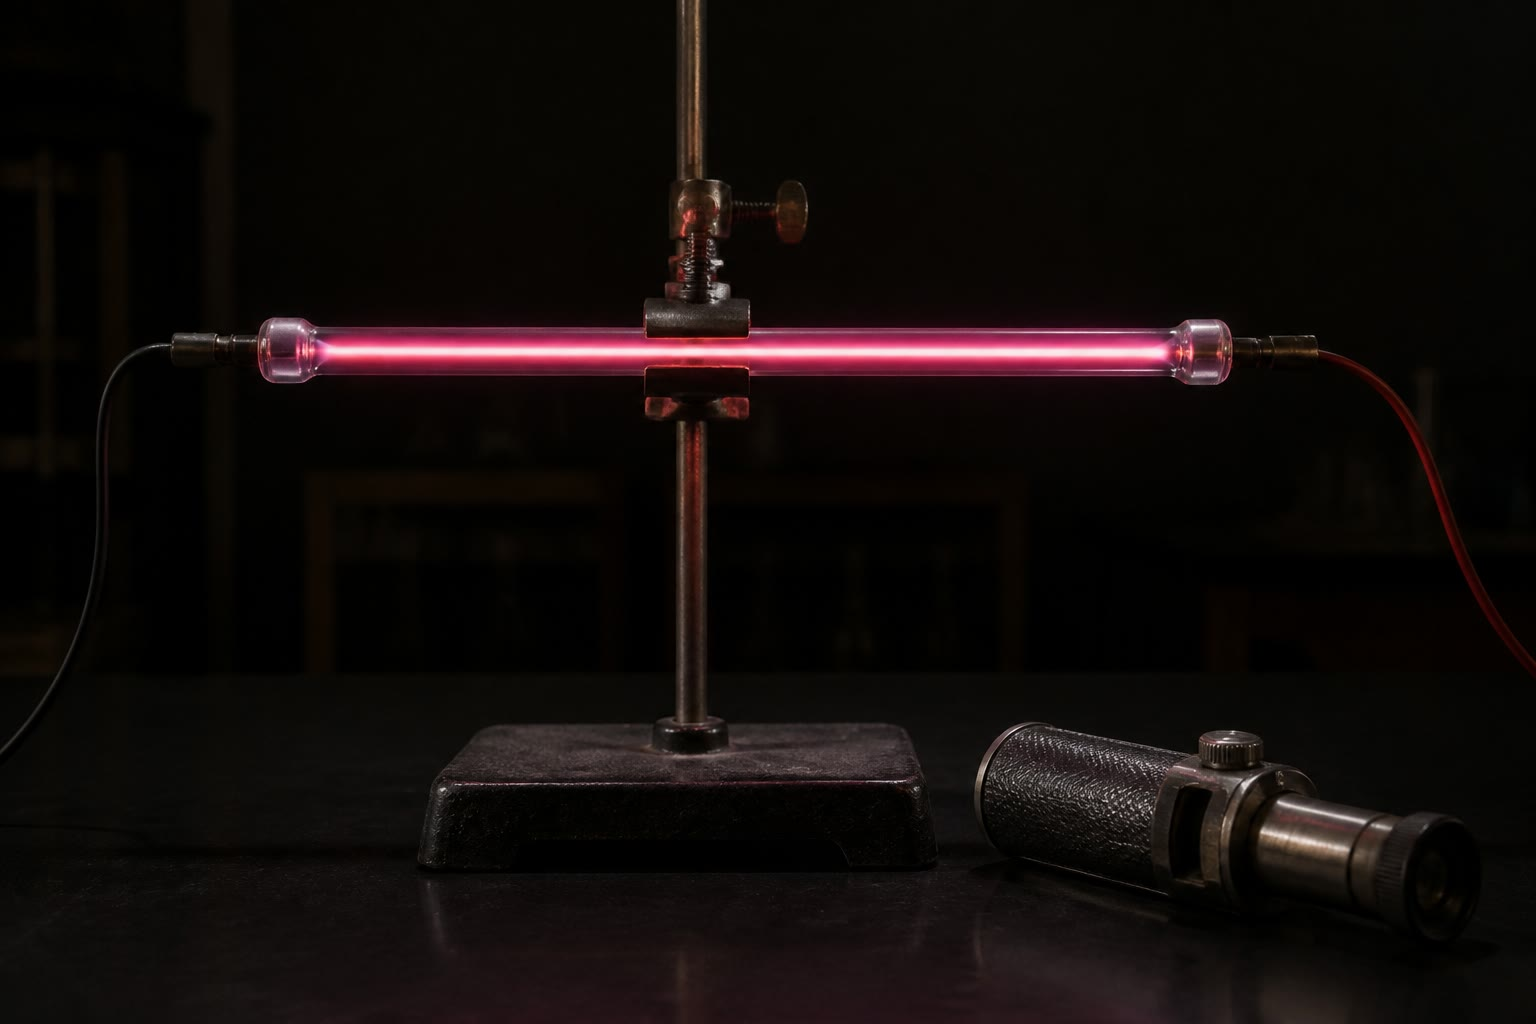
\includegraphics[width=0.58\linewidth]{images/book5/ai/b5-11-discharge-tube.jpg}

{\small Un tube à décharge d'hydrogène et un spectroscope de poche~: la lueur rose, décomposée, devient les raies de Balmer --- l'empreinte entière que ce chapitre déduit du potentiel coulombien.}
\end{omfigure}

\section{Exercices}

\begin{exercise}[$\star$]\label{exo:b3:hydrogen-atom:1}
(a) Vérifier par substitution que $u = Cr\eu^{-r/a_0}$ résout
l'\omterm{prop:b3:schrodinger-three-dimensions:swave}{équation radiale} $l = 0$ avec $E = -E_{\text{I}}$, pourvu que $a_0 =
\hbar^2/m_{\text{e}}k$. (b) La normaliser ($\int_0^\infty
x^2\eu^{-x}\dd x = 2$). (c) Vérifier les dimensions de $a_0$ et de
$E_{\text{I}}$. (d) Pourquoi n'existe-t-il aucun état sous
$-E_{\text{I}}$ (argumenter avec
\cref{exo:b3:schrodinger-three-dimensions:12})~?
\end{exercise}

\begin{exercise}[$\star$]\label{exo:b3:hydrogen-atom:2}
Calculer (a) les longueurs d'onde de Lyman $\alpha$ et de la limite de
Lyman~; (b) les trois premières raies de Balmer et la limite de Balmer
--- lesquelles sont visibles, et de quelles couleurs~? (c) l'étendue
de la série de Paschen~; (d) la fréquence de la transition
$n = 110 \to 109$.
\end{exercise}

\begin{exercise}[$\star$]\label{exo:b3:hydrogen-atom:3}
Pour l'état fondamental~: (a) situer le maximum de $P_{1s}(r)$~; (b)
calculer $\langle r\rangle$~; (c) calculer la probabilité de trouver
l'électron au-delà de $2a_0$ ($\int_x^\infty t^2\eu^{-t}\dd t = (x^2 +
2x + 2)\eu^{-x}$)~; (d) pourquoi les images d'«~orbite~» de rayon
exactement $a_0$ sont-elles trompeuses~?
\end{exercise}

\begin{exercise}[$\star$]\label{exo:b3:hydrogen-atom:4}
(a) Énumérer les couples $(l, m)$ de $n = 3$ et vérifier le compte $n^2 =
9$. (b) Avec le spin, combien d'états dans les couches $n = 1, 2, 3$~?
(c) Les rapprocher des longueurs $2, 8, 18$ des lignes du tableau
périodique. (d) Quelle dégénérescence (en $m$ ou en $l$) survit pour
l'électron externe du sodium, et pourquoi l'autre se brise-t-elle~?
\end{exercise}

\begin{exercise}[$\star\star$]\label{exo:b3:hydrogen-atom:5}
L'échelle de Moseley. Un électron interne (couche K) d'un élément $Z$
se meut dans un champ nucléaire presque nu, écranté par l'unique autre
électron K~: charge effective $\approx Z - 1$. (a) Montrer que
l'énergie du rayon X $2p \to 1s$ vaut approximativement
$\tfrac34(Z-1)^2E_{\text{I}}$. (b) L'évaluer pour le cuivre
($Z = 29$) et comparer à la raie K$\alpha$ mesurée à \qty{8.05}{keV}.
(c) Moseley (1913) traça $\sqrt{\nu}$ en fonction de $Z$ et obtint des
droites~: qu'a prouvé cela sur le sens du numéro atomique~? (d)
Prédiser l'énergie K$\alpha$ de l'élément $Z = 43$, alors manquant.
\end{exercise}

\begin{exercise}[$\star\star$]\label{exo:b3:hydrogen-atom:6}
Le positronium. (a) Justifier $\mu = m_{\text{e}}/2$ et donner son
énergie de liaison et son \omterm{thm:b3:hydrogen-atom:levels}{rayon de Bohr}. (b) Sa longueur d'onde
Lyman $\alpha$. (c) Le para-positronium s'annihile en deux photons~:
leurs énergies et leurs directions relatives (d'après
\cref{ch:b3:relativistic-dynamics}). (d) Où la médecine détecte-t-elle
exactement cette signature chaque jour~?
\end{exercise}

\begin{exercise}[$\star\star$]\label{exo:b3:hydrogen-atom:7}
Les excitons. Dans l'arséniure de gallium,
$\varepsilon_{\text{r}} = 12.9$ et la masse effective réduite vaut
$\mu = 0.058\,m_{\text{e}}$. (a) Montrer que
$a_{\text{ex}} = a_0\,\varepsilon_{\text{r}}\,m_{\text{e}}/\mu$ et
l'évaluer. (b) L'énergie de liaison de l'exciton. (c) Comparer
$a_{\text{ex}}$ aux rayons de boîte quantique de
\cref{pb:b3:schrodinger-three-dimensions:1} et justifier enfin la
négligence du terme de Coulomb dans les petites boîtes. (d) Pourquoi
les raies excitoniques n'apparaissent-elles que dans des
semi-conducteurs \emph{purs et froids} ($k_{\text{B}}T$ face à votre
réponse à (b))~?
\end{exercise}

\begin{exercise}[$\star\star$]\label{exo:b3:hydrogen-atom:8}
Pénétration et métaux alcalins. Le sodium est un électron de valence
hydrogénoïde à l'extérieur d'un cœur fermé de charge effective $+e$.
(a) Lequel de $3s$, $3p$, $3d$ ressent le plus le noyau incomplètement
écranté, et pourquoi (rappeler la figure radiale)~? (b) Les
niveaux mesurés sont $E_{3s} = \qty{-5.14}{eV}$, $E_{3p} = \qty{-3.04}{eV},
E_{3d} = \qty{-1.52}{eV}$~: vérifier que $3d$ est presque hydrogénoïde
($n = 3$) alors que $3s$ est bien plus profond, et expliquer. (c)
Calculer la longueur d'onde de $3p \to 3s$~: quelle couleur célèbre
est-ce~? (d) Écrire les niveaux alcalins sous la forme
$-E_{\text{I}}/(n - \delta_l)^2$ et extraire les «~défauts
quantiques~» $\delta_s$ et $\delta_p$ du sodium.
\end{exercise}

\begin{exercise}[$\star\star$]\label{exo:b3:hydrogen-atom:9}
Un proton d'une nébuleuse capture un électron dans $n = 100$. (a)
Quelle énergie est libérée dans le photon de capture si l'électron
arrivait presque libre~? (b) L'atome dégringole, de préférence par
pas $\Delta n = 1$ aux $n$ élevés~: dans quelle bande tombent ces
photons~? (c) La dernière étape de la cascade est Lyman $\alpha$~; la
lumière visible des nébuleuses est dominée par H$\alpha$~: repérer de
quelle étape de la cascade il s'agit. (d) Expliquer pourquoi les
nébuleuses en émission luisent en \emph{rouge} alors que la raie la
plus intense de l'hydrogène (Lyman $\alpha$) est ultraviolette.
\end{exercise}

\begin{exercise}[$\star\star\star$]\label{exo:b3:hydrogen-atom:10}
Moyennes et viriel. Pour l'état fondamental, calculer (a)
$\langle 1/r\rangle$ et vérifier $\langle E_p\rangle = -2E_{\text{I}}
= 2E_1$~; (b) $\langle E_k\rangle = +E_{\text{I}}$, ce qui vérifie le
rapport du viriel de \cref{exo:b3:hamiltonian-mechanics:4}~; (c) la
vitesse quadratique moyenne de l'électron et $v/c$~; (d) l'ordre de grandeur du champ magnétique que le
\emph{proton} subit du fait du mouvement de l'électron (une boucle de
courant $ev/2\pi a_0$ vue à la distance $a_0$) --- un nombre dont la
structure hyperfine aura besoin.
\end{exercise}

\begin{exercise}[$\star\star\star$]\label{exo:b3:hydrogen-atom:11}
À quel point la structure fine est-elle fine. (a) Montrer que
l'échelle de vitesse de l'état fondamental est
$\langle v^2\rangle^{1/2}/c = \alpha \approx 1/137$, et pour un
hydrogénoïde de charge $Z$~: $Z\alpha/n$. (b) Les corrections
relativistes entrent à l'ordre relatif $(v/c)^2$~: estimer l'échelle
de structure fine $\alpha^2E_{\text{I}}$ en meV, et l'ordre de
grandeur de l'écart pour $n = 2$ en GHz. (c) Pour l'uranium
hydrogénoïde ($Z = 92$)~: $v/c$ à $n = 1$ --- le traitement non
relativiste est-il tenable~? (d) Qu'annonce physiquement la
divergence formelle en $Z\alpha \to 1$ ($Z \approx 137$)~?
\end{exercise}

\begin{exercise}[$\star\star\star$]\label{exo:b3:hydrogen-atom:12}
La dégénérescence déraisonnable. (a) En mécanique classique, montrer
que pour $V = -k/r$ l'orbite se referme (pas de précession) en
invoquant le vecteur conservé de Laplace--Runge--Lenz $\vect A = \vect p\wedge\vect
L - mk\,\vect e_r$ --- vérifier $\dd\vect A/\dd t = 0$ avec la loi de
Newton. (b) Argumenter~: un vecteur conservé qui fixe l'axe de
l'ellipse est une symétrie supplémentaire au-delà des rotations ---
et symétrie supplémentaire signifie dégénérescence supplémentaire
(rappeler \cref{exo:b3:quantum-formalism:9}). (c) Ajouter une
petite correction en $1/r^2$ au potentiel et montrer que l'ellipse
précesse~: l'axe tourne, $\vect A$ n'est plus conservé. (d)
Relier~: dans les atomes polyélectroniques le potentiel effectif n'est
pas en $1/r$ pur, et la dégénérescence en $l$ se brise (le sodium~!)~;
dans l'hydrogène même, la relativité fournit la petite correction ---
de quel trait observé de \cref{exo:b3:hydrogen-atom:11} s'agit-il~?
\end{exercise}

\section{Problème~: des atomes géants}

\begin{problem}[{Problème du week-end --- les atomes de Rydberg, de la
lueur radio de la Galaxie aux ordinateurs quantiques}]\label{pb:b3:hydrogen-atom:1}
Étirer l'hydrogène jusqu'à $n \approx 100$ et il devient un objet
d'une autre espèce~: large de quelques micromètres, lié par des
millielectronvolts, absurdement sensible --- et absurdement utile. Ce
problème réétalonne vers le haut la solution de l'hydrogène, d'abord
vers les nuages interstellaires qui émettent aux longueurs d'onde
centimétriques, puis vers les réseaux de laboratoire où de tels géants
s'intriquent en processeurs. Données~:
$E_{\text{I}} = \qty{13.6}{eV}$, $a_0 = \qty{52.9}{pm}$,
$R_{\text{H}}c = \qty{3.29e15}{Hz}$, $k_{\text{B}}T$ à
\qty{300}{K} vaut \qty{25.9}{meV}.

\medskip\noindent\textbf{Partie I --- Les lois d'échelle.}
\begin{enumerate}
  \item Donner les quatre lois d'échelle de base en $n$~: taille $\langle
        r\rangle$, liaison $|E_n|$, écart $E_{n+1} - E_n$ (aux grands
        $n$) et fréquence orbitale classique de l'orbite de Bohr
        correspondante.
  \item Montrer qu'aux grands $n$ la fréquence de transition $n+1 \to
        n$ tend vers $2R_{\text{H}}c/n^3$, et vérifier qu'elle égale
        la fréquence orbitale classique (le principe de
        correspondance de \cref{pb:b3:hamiltonian-mechanics:1},
        achevé).
  \item Évaluer taille et liaison à $n = 50$ et $n = 100$.
  \item Le dipôle électrique d'un atome de Rydberg varie comme
        $n^2ea_0$~: l'évaluer à $n = 50$ en debyes ($1\,\text{D} =
        \qty{3.34e-30}{C.m}$) et comparer au \qty{1.85}{D} d'une
        molécule d'eau.
  \item Estimer le champ électrique qui déchire l'atome $n = 50$,
        sous la forme $F \sim |E_n|/(e\,\langle r\rangle)$, en V/cm.
  \item Pourquoi de tels atomes ne survivent-ils pas à la chimie d'un
        vide de laboratoire ordinaire --- alors qu'ils survivent fort
        bien dans l'espace interstellaire (comparer les taux de
        collision)~?
\end{enumerate}

\medskip\noindent\textbf{Partie II --- Les raies de recombinaison de
la Galaxie.}
Dans les nébuleuses ionisées, les protons capturent des électrons à
$n$ élevé~; la cascade rayonne un peigne de «~raies de recombinaison
radio~».
\begin{enumerate}[resume]
  \item Calculer la fréquence de la transition $n = 110 \to 109$
        (appelée H109$\alpha$).
  \item Dans quelle bande tombe-t-elle, et quel type de télescope la
        reçoit~?
  \item Calculer la longueur d'onde de H109$\alpha$ et la comparer à
        la taille de l'atome émetteur~: combien d'atomes tiennent
        dans une longueur d'onde~?
  \item Ces raies mesurent la température de la nébuleuse par leur
        largeur Doppler~: à $T = \qty{e4}{K}$, la vitesse thermique
        de l'hydrogène vaut $\sim\qty{12.8}{km/s}$ --- calculer la
        largeur relative $\Delta\nu/\nu$ et la largeur de
        H109$\alpha$ en kHz.
  \item Les ondes radio traversent la poussière qui noircit le ciel
        optique~: que cela permet-il de cartographier aux astronomes
        des raies de recombinaison, et que les astronomes des raies
        de Balmer ne peuvent pas~?
  \item Au-delà de $n \sim 1000$ environ (des atomes de $0.05$
        millimètre~!), les niveaux se brouillent en un continuum même
        dans l'espace~: nommer deux effets qui élargissent ou
        détruisent de tels états.
\end{enumerate}

\medskip\noindent\textbf{Partie III --- Des géants au laboratoire.}
\begin{enumerate}[resume]
  \item Des lasers portent des atomes de rubidium à $n \approx 70$
        dans des réseaux de pinces optiques espacées d'un micromètre.
        Deux tels atomes distants de $R$ interagissent par leurs
        dipôles induits (rappeler
        \cref{exo:b3:harmonic-oscillator:10})~: avec un dipôle
        $\propto n^2$, montrer que l'intensité de van der Waals varie
        comme un colossal $n^{11}$ (utiliser $C_6 \propto d^4/\Delta E$
        avec un espacement $\Delta E \propto n^{-3}$).
  \item Le «~blocage~»~: à l'intérieur d'un rayon $R_{\text{b}}$,
        l'interaction déplace l'état doublement excité hors de
        résonance du laser, de sorte que \emph{deux} atomes ne
        peuvent pas être excités ensemble. Expliquer en une phrase
        pourquoi cela réalise une porte à deux qubits.
  \item Les rayons de blocage atteignent plusieurs micromètres ---
        des milliers de fois la taille des atomes dans leur état
        fondamental~: pourquoi cette longue portée (à comparer à
        l'échelle nanométrique de la chimie) est-elle exactement ce
        que veut un processeur extensible~?
  \item Un état de Rydberg à $n = 70$ vit $\sim\qty{100}{\micro s}$
        tandis qu'une porte prend $\sim\qty{0.5}{\micro s}$~: combien
        d'opérations tiennent grossièrement dans une durée de vie, et
        pourquoi est-ce ce rapport, et non la durée de vie seule, qui
        importe~?
  \item Le rayonnement du corps noir à température ambiante, dont le
        maximum est vers \qty{100}{meV} mais dont la queue de basse
        énergie est riche, provoque des transitions entre niveaux de
        Rydberg voisins séparés de seulement $\sim\qty{0.1}{meV}$~:
        pourquoi les expériences de précision doivent-elles enfermer
        les atomes dans des écrans froids~?
  \item Estimer combien de transitions dipolaires de type antenne
        ($\propto n^2$) un bain de photons à \qty{300}{K} entraîne
        par seconde, comparé à un atome $n = 1$~: quelle loi
        d'échelle fait des atomes de Rydberg des \emph{capteurs}
        exquis de champs micro-ondes et térahertz~?
\end{enumerate}

\medskip\noindent\textbf{Partie IV --- La vue d'ensemble.}
\begin{enumerate}[resume]
  \item Une seule formule, $E_n = -E_{\text{I}}\mu Z^2/m_{\text{e}}n^2$,
        couvre combien d'ordres de grandeur d'énergie de liaison, de
        l'uranium hydrogénoïde ($Z = 92$, $n = 1$) jusqu'à un état de
        Rydberg $n = 1000$~? Calculer les deux extrémités.
  \item Les durées de vie radiatives des états de $l$ faible varient
        comme $n^3$~: à partir de la durée de vie de $2p$,
        \qty{1.6}{ns}, estimer celle d'un état $100p$ --- et
        comparer au problème du corps noir à température ambiante de
        la partie III.
  \item Au CERN, des anti-atomes d'antihydrogène sont désormais
        spectroscopiés sur l'intervalle $1s \to 2s$ à quinze
        chiffres~: quelle symétrie fondamentale l'accord avec
        l'hydrogène ordinaire teste-t-il, et pourquoi l'hydrogène
        est-il le bon atome pour cette comparaison~?
  \item À $n \sim 100$ l'onde de de Broglie de l'électron enroule une
        orbite presque classique~; à $n = 1$ aucune orbite n'existe~:
        en une phrase, où l'image classique s'allume-t-elle~?
  \item La constante de Rydberg est mesurée à quinze chiffres~:
        pourquoi l'hydrogène est-il, entre tous les systèmes, l'ancre
        naturelle de précision de la physique atomique~?
  \item Le prix Nobel 2012 (Haroche) a utilisé des atomes de Rydberg
        comme compteurs de photons qui ne détruisent pas le photon~:
        quelles deux propriétés des parties I et III en font des
        sondes non destructives idéales des champs micro-ondes~?
  \item Résumer le résultat nommé~: les lois d'échelle en $n^2$,
        $n^{-2}$, $n^{-3}$ et $n^{11}$ d'un unique atome résolu
        exactement étirent l'hydrogène de \qty{52.9}{pm} à un
        demi-micromètre, accordent sa voix de \qty{121.6}{nm} à
        \qty{6}{cm}, et en font à la fois la balise radio de la
        Galaxie et la porte à deux qubits des ordinateurs quantiques
        à atomes neutres.
\end{enumerate}
\end{problem}
